\section{Algorithm}
\label{sec:algorithm}

In this section we describe our ROSC algorithm. Figure~\ref{figure:flow_graph}(c) shows a 
flow diagram of ROSC. ROSC follows the basic pipeline of spectral clustering except that
it generates a coefficient matrix $Z$ 
%(shown in the red box of the diagram) 
and feeds it
 into the clustering pipeline in place of
the similarity matrix $S$. 
The objective is to find a  $Z$ that possesses  grouping effect. 
To achieve that, ROSC uses PI to obtain {\pev}s from which a basic $Z$ is derived.
Next, it generates the TKNN graph with which $Z$ is rectified. 
In the following, we discuss how $Z$ is derived from the {\pev}s, define the TKNN graph,
describe the rectification process, 
and prove that the resulting $Z$ has the desired grouping effect. 

%
%In this section, we propose a \textbf{RO}bust \textbf{S}pectral \textbf{C}lustering method ROSC. 
%Instead of directly performing spectral clustering on the given similarity matrix, 
%it constructs a new matrix that reserves the efficacy of effective similarities 
%and rectifies ineffective ones in the raw similarity matrix.
%The new matrix will lead to a more robust spectral clustering.

\comment{
\subsection{Model overview}
The overall framework of ROSC is summarized as follows.

First, generate a set of pseudo-eigenvectors.
Since the standard spectral clustering methods using only the dominant eigenvectors may fail 
in the data containing multi-scale clusters,
we generate a set of pseudo-eigenvectors to fuse more useful cluster-separation information.

Second, rectify the given similarity matrix.
The failure of spectral clustering on multi-scale data originates from the inaccurate similarity matrix.
Therefore, we rectify the matrix and aim to achieve a new one
that can more accurately reflect the true similarities between objects.
%This is a major problem to be addressed.

Third, perform spectral clustering.
After rectification, the new similarity matrix will be more accurate and it will be safer to perform spectral clustering. 

These three steps will lead to robust clustering results and next we introduce each step in detail.
}

\subsection*{Pseudo-Eigenvectors}
\label{sec:sec:pseudo}
Given a similarity matrix $S$, we normalize it by $D^{-1}S$ and apply PI to obtain {\pev}s.
%When dealing with multi-scale data,
%spectral clustering
%using only the top-$k$ eigenvectors may fail while some other eigenvectors may be useful~\cite{lin2010power}.
%Therefore, it is necessary to fuse the discriminative cluster-separation information in all eigenvectors
%and PI provides such fusion by returning a pseudo-eigenvector.
%However, when the number of clusters is large,
%a single pseudo-eigenvector is insufficient due to the cluster-collision problem. 
%%Since PI returns a pseudo-eigenvector that is a combination of all the eigenvectors,
Similar to~\cite{ye2016fuse},
we run PI multiple times with different random initial vectors to generate a set of {\pev}s, 
which maps each object into a low dimensional embedding.
Note that small {\ev}s are {\it shrunk} by PI~\cite{lin2010power}.
%\footnote{From Equation~\ref{eq:pi}, we see that the $i$-th 
%largest \ev\ is 
%shrunk at a rate of $\lambda_i/\lambda_1$ per iteration.}.
To alleviate the shrinkage of small {\ev}s,
we follow the approach of~\cite{huang2014diverse}
and gradually decrease the number of iterations executed in PI as more {\pev}s are obtained. 

Since the {\pev}s approximate the most dominant {\ev}, they could be similar. 
To reduce this redundancy,
whitening~\cite{kessy2017optimal} is used to make the pseudo-eigenvectors uncorrelated.
Moreover, noise in the {\pev}s are reduced 
by a rectification process, which will be discussed later.

\comment{
First, we generate a set of pseudo-eigenvectors using different random vectors $\bm{v}_0$.
From Eq.~\ref{eq:v0}, $\bm{v}_0$ can be represented by the subspace spanned by all the eigenvectors.
Suppose $\bm{e}_i$ is an informative eigenvector with a relatively small eigenvalue $\lambda_i$.
Given a $\bm{v}_0$, if it has a dominant component in the direction of $\bm{e}_i$, 
i.e., the associated coefficient $c_i$ is large, 
with an appropriate number of iterations, $c_i\lambda_i^t\approx c_2\lambda_2^t$,
the effect of $\bm{e}_i$ will be finally retained in the pseudo-eigenvector.
Therefore, multiple pseudo-eigenvectors generated by different $\bm{v}_0$
may increase the chance to hold all the informative eigenvectors.

Second, we can control the number of iterations in PI.
In PIC, the \emph{velocity} and \emph{acceleration} at the $t$-th iteration are respectively defined as
$\bm{\delta}_t = \bm{v}_t - \bm{v}_{t-1}$ and $\bm{\epsilon}_t = \bm{\delta}_t-\bm{\delta}_{t-1}$.
A threshold $\epsilon$ is introduced to measure the acceleration change in two consecutive iterations 
and stop PI when $|\bm{\epsilon}_t-\bm{\epsilon}_{t-1}|<\epsilon$.
However,
since the effect of eigenvectors corresponding to smaller eigenvalues will shrink as $t$ increases,
we can decrease the number of iterations by gradually increasing the $\epsilon$ value,
which provides another way to keep useful information in ``less important'' eigenvectors. 
}

\subsection*{Transitive {\it K} Nearest Neighbor (TKNN) Graph}

%\begin{figure}
%    \centering
%        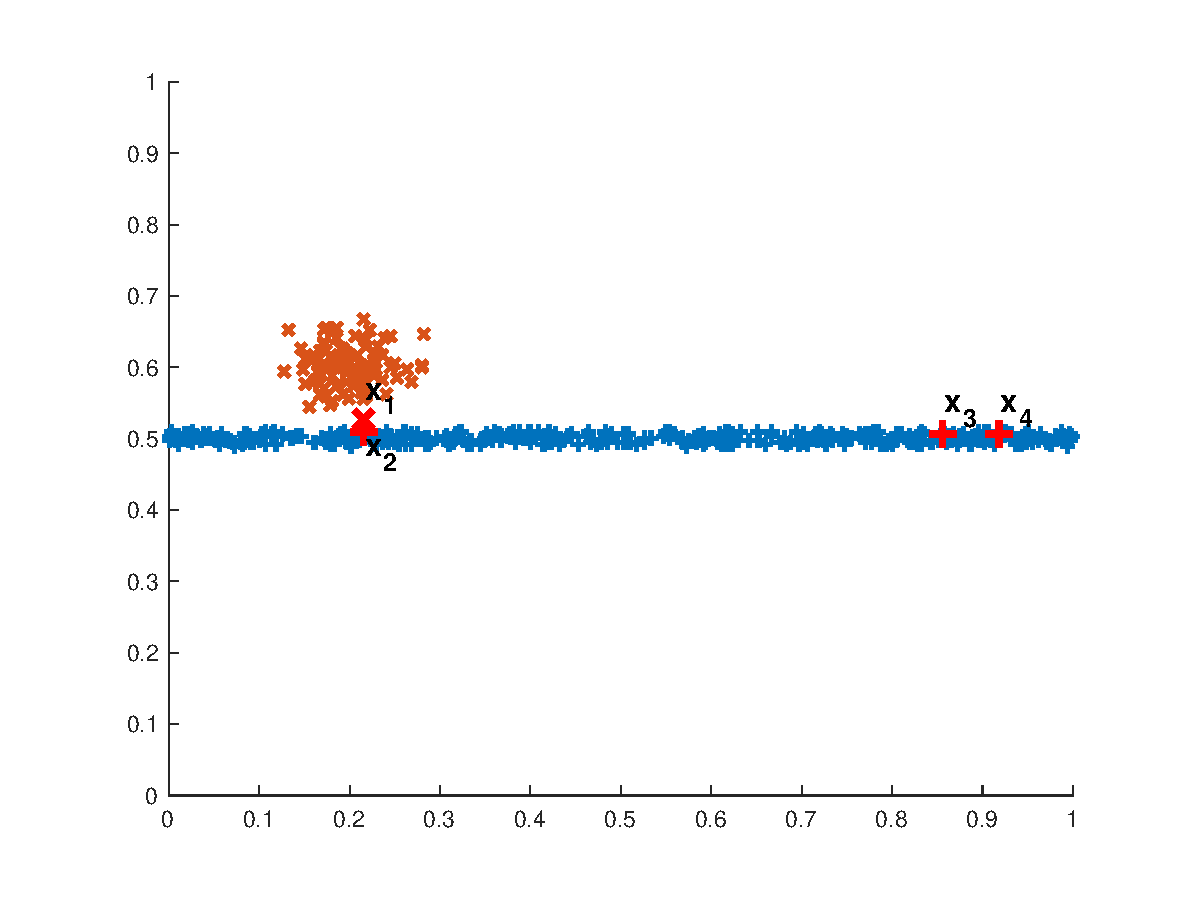
\includegraphics[width = 0.8\linewidth]{figure/example1.eps}
%        \caption{An toy example}
%        \label{figure:example1}
%\end{figure}

%The \emph{$K$ nearest neighbor} (KNN) graph is generally used to depict the most adjacent relations between objects,
%in which the linked objects are generally assumed to share common characteristics.
%Given a set of objects $\mathcal{X} = \{\bm{x}_1,\bm{x}_2,...,\bm{x}_n\}$,
%the KNN graph $G_{K} = (V, E)$ is a graph with $V = \mathcal{X}$ and $E = \{e_{ij}\}$.
%%An edge $e_{ij}$ between $\bm{x}_i$ and $\bm{x}_j$ indicates
%%$x_j \in N_K(\bm{x}_i)$ or $x_i \in N_K(\bm{x}_j)$,
%%where $N_K(\bm{x}_i)$ denotes the set of $K$ nearest neighbors of $\bm{x}_i$.
%%at least one of the two end nodes is in the $K$ nearest neighborhood of the other.
%%However, the $K$ nearest neighborhood relation is not symmetric,
%%i.e., $x_j \in N_K(\bm{x}_i)$ is inequivalent to $x_i \in N_K(\bm{x}_j)$, 
%Some previous work~\cite{yin2016laplacian} simply considers $e_{ij}$
%exists when $\bmx_j \in N_K(\bmx_i)$ or $x_i \in N_K(\bmx_j)$,
%where $N_K(\bmx_i)$ denotes the set of $K$ nearest neighbors of $\bmx_i$.
%However,
%in the case of data containing multi-scale clusters,
%such definition may lead to an edge between
%two objects in different clusters.
%Fig.~\ref{figure:example1} shows an toy example which consists of two multi-scale clusters
%marked by ``$\times$" and ``$+$" respectively.
%For object $\bmx_1$,
%object $\bmx_2$ is its nearest neighbor.
%But for $\bmx_2$, $\bmx_1$ is far away from it.
%In this case, there will be an edge between $\bmx_1$ and $\bmx_2$ in the traditional KNN graph.
%However, since $\bmx_1$ and $\bmx_2$ belong to different clusters,
%they should not be connected.

Our objective is to capture the high correlations between objects that belong to the same cluster even 
 though the objects could be located at distant far ends of a cluster. 
 These correlations are expressed via a TKNN graph, which is used to 
 regularize the coefficient matrix $Z$.

\begin{definition}
\label{def:nei_relation}
\textbf{(Mutual  $K$-nearest neighbors)}
Let $N_K(x)$ be the set of $K$ nearest neighbors of an object $x$.
Two objects $x_i$ and $x_j$ are said to be mutual $K$-nearest neighbors of each other,
denoted by $x_i \sim x_j$, 
iff $x_i \in N_K(x_j)$ and $x_j \in N_K(x_i)$.
\hfill$\Box$
\end{definition}

%In the case of multi-scale data,
%the KNN graph is sometimes insufficient to reflect whether two objects belong to the same cluster or not.
%For example, objects $\bmx_2$ and $\bmx_3$ in Fig.~\ref{figure:example1} belong to the same cluster, 
%but they are both far away from each other.
%%objects $x_1$ and $x_2$ are in different clusters despite their closeness.
%To construct an effective KNN graph, $\bmx_2$ and $\bmx_3$
%are expected to be linked.
%Therefore,
%the reachability between two objects is introduced.

\begin{definition}
\label{def:reachability}
\textbf{(Reachability)}
Two objects $x_i$ and $x_j$ are said to be reachable from each other
if there exists a sequence of $h \geq 2$ objects 
 $\{x_i = x_{a_1}, \ldots, x_{a_h} = x_j\}$ such that
 $x_{a_r} \sim x_{a_{r+1}}$ for $1 \leq r < h$.
 \hfill$\Box$
\end{definition}

\begin{definition}
\label{def:trans_relation}
\textbf{(Transitive $K$-nearest neighbor (TKNN) graph)}
Given a set of objects $\mathcal{X} = \{x_1, x_2,..., x_n\}$,
the TKNN graph $\mathcal{G}_K = (\mathcal{X},\mathcal{E})$
is an undirected graph
where $\mathcal{X}$ is the set of vertices and $\mathcal{E}$ is the set of edges.
Specifically, the edge ($x_i$, $x_j$) $\in \mathcal{E}$
iff $x_i$ and $x_j$ are reachable from each other.
We represent the TKNN graph by an $n \times n$ {\it reachability matrix}
$\mathcal{W}$ 
whose ($i$,$j$)-entry $\mathcal{W}_{ij} = 1$ if ($x_i$, $x_j$) $\in \mathcal{E}$; 0 otherwise.
\hfill$\Box$
\end{definition}

%We note that mutual-KNN is a symmetric relation and so is reachability. 

%Compared with the traditional KNN graph, 
%the TKNN graph can more accurately reflect 
%whether two objects belong to the same cluster or not.
%It will be used in the next section to rectify the matrix of similarity between objects.
 
\subsection*{Coefficient Matrix}
%In the case of multi-scale data,
%the distance-based similarity is likely to be ineffective. 
%To improve the clustering performance,
%it is necessary to rectify the matrix.
%The rectification should follow two principles.
%First, for the effective similarities, the efficacy should be reserved.
%Second, for the ineffective ones, the efficacy should be enhanced.
%For example,
%the closeness between objects $\bmx_3$ and $\bmx_4$ in Fig.~\ref{figure:example1}
%leads to a large similarity value.
%Since the two objects are of the same cluster,
%the new value should still be large.
%In comparison, 
%both the similarity between $\bmx_1$ and $\bmx_2$ and the one between $\bmx_2$ and $\bmx_3$
%should be rectified, as these distance-based similarities are ineffective.

%In the multi-scale data,
%different clusters may have different sizes, densities or even geometric structures.
The similarity between two objects describes the degree to which they share common characteristics.
The more similar they are, 
the more likely that one object can be represented by the other. 
Therefore,
to depict the relationships between objects in multi-scale data,
each object is linearly characterized by other objects,
assuming the well-known linear subspace model~\cite{liu2013robust}.

We generate $p$ {\pev}s using PI. 
%just as a non-linear manifold can be locally approximated by linear subspaces.
%First, these vectors, which retain the effects of dominant eigenvectors,
%can certainly retain the original accurate similarities between objects.
%Second, they absorb the cluster-separation information from the seemingly ``less important'' eigenvectors,
%which further provides a reliable source of information to rectify the erroneous similarities.
Let $X\in \mathcal{R}^{p\times n}$ be a matrix whose rows are the {\pev}s.
The $q$-th column of $X$ can be taken as a feature vector $\bmx_q$ of an object $x_q$.
We normalize the column vectors of $X$ such that $\bmx_q^T \bmx_q = 1 \; \forall 1 \leq q \leq n$.
We determine a coefficient matrix $Z \in \mathcal{R}^{n \times n}$ by\footnote{We will regularize $Z$ to avoid the trivial solution of $Z$ being the identity matrix.}
\begin{equation}
\label{eq:nonoise}
%X = XZ,\;\;\; \text{s.t. } diag(Z) = 0.
X = XZ.
\end{equation} 
One can interpret $Z_{ij}$ 
as a value that reflects how well object $x_i$ characterizes object $x_j$.
%To avoid the trivial solution of $Z$ equalling the identity matrix,
%we will regularize $Z$ later.
%For simplicity, we do not explicitly mention this constraint in the rest of the paper.

As indicated by previous works~\cite{ye2016fuse}, the generated pseudo-eigenvectors are likely to be noise-corrupted.
We thus extend Equation~\ref{eq:nonoise} by introducing a noise matrix $O$, giving:
%However, although the pseudo-eigenvectors inherit useful cluster-separation information,
%they may also be contaminated by noise.
%Thus a matrix $O$ is introduced to capture the noise,
\begin{equation}
X = XZ + O.
\label{eq:O}
\end{equation} 
%The TKNN graph conveys information on whether two objects belong to the same cluster or not,

As we have explained, the TKNN graph  conveys useful clustering information, bringing highly
correlated objects that are located at distant far ends of a cluster together.
We thus use the TKNN graph to regularize matrix $Z$.
We derive the following objective function:
%Since our objective is to derive a $Z$ which can better reflect the true similarities between objects,
\comment{
\begin{equation}
%\label{eq:obj}
\min_Z ||O||_F^2+\lambda_1||Z||_F^2 + \lambda_2||Z-\mathcal{W}_K||_F^2,
s.t., X = XZ+O,
\end{equation}
}
%By substituting $O$, we derive
\begin{equation}
\label{eq:obj_constraint}
\min_Z ||X-XZ||_F^2 + \alpha_1 ||Z||_F^2 + \alpha_2 ||Z-\mathcal{W}||_F^2,
\end{equation}
where $\alpha_1 > 0,\alpha_2 \geq 0$ are two 
weighting factors that adjust the relative weights of the three components that constitute
the objective function.
The objective function consists of three terms.
The first term aims to reduce the noise matrix $O$ (see Equation~\ref{eq:O}),
the second term is the Frobenius norm on $Z$, and
%that restricts any item in $Z$ from being dominant.
the third term regularizes $Z$ by the TKNN graph.
%For simplicity, as in~\cite{lu2012robust},
%we remove the constraint and formulate the problem as
%\begin{equation}
%\label{eq:obj}
%\min_Z ||X-XZ||_F^2 + \lambda_1 ||Z||_F^2 + \lambda_2 ||Z-\mathcal{W}_K||_F^2.
%\end{equation}
%$\lambda_1$ and $\lambda_2$ are two parameters to balance the effects of three parts.
A closed-form solution, $Z^*$, to the optimization problem is
\begin{equation}
\label{eq:solution}
Z^* = (X^TX + \alpha_1I + \alpha_2I)^{-1}(X^TX+\alpha_2\mathcal{W}).
\end{equation}

\subsection*{Grouping Effect}
For an object $x_p$, 
let $\bmz_p$ be the $p$-th column of the coefficient matrix $Z$.
We interpret the entries of $\bmz_p$ as the coefficients that express $x_p$ as a linear combinations
of other objects. 
Previous works~\cite{lu2012robust,lu2013correlation,hu2014smooth} have shown that if $Z$ has {\it grouping effect}, then performing spectral 
clustering based on $Z$ would be effective. 
Intuitively, $Z$ has grouping effect if, given two {\it highly correlated} objects $x_i$ and $x_j$,
their characterizations of other objects are similar.
Existing works mostly consider {\it high correlation} between objects as {\it high similarity} of their
feature vectors. With ROSC, we consider object similarity in terms of both feature similarity and 
reachability similarity. 
Feature similarity is measured by the objects' feature vectors as given by the columns of matrix $X$.
Reachability similarity is measured by the columns of matrix $\mathcal{W}$, 
each of which shows the reachability of an object to all others. 
Formally,



%It has been shown that the first two terms in the objective function decide the \emph{grouping effect} of $Z$~\cite{lu2012robust}.
%In Problem~\ref{eq:obj}, the first two terms decides whether $Z$ has the grouping effect~\cite{lu2012robust} defined as follows.
%i.e., the more highly correlated two objects are,
%the larger weight one will have in characterizing the other~\cite{lu2012robust}.

\begin{definition}
\label{def:grouping}
\textbf{(Grouping effect)}. 
Given a set of objects $\mathcal{X} = \{x_1, x_2,..., x_n\}$,
let $\bmw_q$ be the $q$-th column of $\mathcal{W}$. 
Further, let $\xarrow{i}{j}$ denote the condition:
(1) $\bmx_i^T \bmx_j \rightarrow 1$ and 
(2) $\lVert \bmw_i - \bmw_j \rVert_2 \rightarrow 0$.
A matrix $Z$ is said to have grouping effect
if
\[
\xarrow{i}{j} \Rightarrow |Z_{ip} - Z_{jp}| \rightarrow 0\; \forall 1 \leq p \leq n.
\]
%for an arbitrary object $\bmx$ and its associated coefficient vector $\bm{z}$,
%If $\bmx_i\rightarrow \bmx_j$,
%then $z_{pi}\rightarrow z_{pj}$,
%where $z_{pi}$ and $z_{pj}$ are the $i$th and $j$th entry in $\bm{z}_p$ respectively.
%Then we say the self-representation matrix $Z$
%has the grouping effect.
%\hfill$\Box$
\end{definition}

Our next task is to prove that the optimal solution $Z^*$ (as given in Equation~\ref{eq:solution})
% of Equation~\ref{eq:obj_constraint}
has the grouping effect.
In the following discussion, we use $\bmz_q^*$ to denote the $q$-th column vector of $Z^*$.

\begin{lemma}
\label{lemma1}
Given a set of objects $\mathcal{X}$,
the matrix
$X\in \mathcal{R}^{p\times n}$ that is composed of the {\pev}s as rows,
 the reachability matrix $\mathcal{W}$,
 and the optimal soution $Z^*$ of Equation~\ref{eq:obj_constraint},
\begin{equation}
\label{eq:zi}
Z_{ip}^* = \frac{\bm{x}_i^T(\bm{x}_p-X\bm{z}_p^*) + \alpha_2 \mathcal{W}_{ip}}{\alpha_1+\alpha_2}, \;\;\; \forall 1 \leq i, p \leq n.
\end{equation}
\end{lemma}

\begin{proof}
For $1 \leq p \leq n$,
let $J(\bm{z}_p) =  ||\bm{x}_p-X\bm{z}_p||_2^2 + \alpha_1 ||\bm{z}_p||_2^2 + \alpha_2 ||\bm{z}_p-\bm{w}_p||_2^2$.
Since $Z^*$ is the optimal solution of Equation~\ref{eq:obj_constraint}, we have $\frac{\partial{J}}{\partial{Z}_{ip}}|_{\bm{z}_p = \bm{z}_p^*} = 0\; \forall 1\leq i \leq n$.
Hence, $-2\bm{x}_i^T(\bm{x}_p-X\bm{z}_p^*)+2\alpha_1Z_{ip}^*+2\alpha_2(Z_{ip}^*-\mathcal{W}_{ip}) = 0$,
which induces Equation~\ref{eq:zi}.
\end{proof}

%\begin{lemma}
%\label{lemma1}
%Given a set of objects $X\in \mathcal{R}^{d\times n}$ and a TKNN graph $\mathcal{G} = (\mathcal{V}, \mathcal{E}, \mathcal{W}_K)$,
%let $\bm{x}_p$ be an arbitrary object and $\bm{w}_p$ be the column vector in $\mathcal{W}_K$ describing the connectivity of $\bmx_p$.
%Each item $z_{pi}^*$ in the optimal solution $\bm{z}_p^*$ to the problem 
%$\min_{\bm{z}} ||\bm{x}_p-X\bm{z}_p||_2^2 + \lambda_1 ||\bm{z}_p||_2^2 + \lambda_2 ||\bm{z}_p-\bm{w}_p||_2^2$ is
%\begin{equation}
%\label{eq:zi}
%z_{pi}^* = \frac{\bm{x}_i^T(\bm{x}_p-X\bm{z}_p^*) + \lambda_2 w_{pi}}{\lambda_1+\lambda_2},
%\end{equation}
%where $w_{pi} = 1$, if $\bm{x_p}$ and $\bm{x}_i$ are reachable; $0$, otherwise. 
%
%Proof. Let $J(\bm{z}_p) =  ||\bm{x}_p-X\bm{z}_p||_2^2 + \lambda_1 ||\bm{z}_p||_2^2 + \lambda_2 ||\bm{z}_p-\bm{w}_p||_2^2$.
%Since $\bm{z}_p^*$ is the optimal solution, then $\frac{\partial{J}}{\partial{z}_{pi}}|_{\bm{z}_p = \bm{z}_p^*} = 0$.
%Thus we have $-2\bm{x}_i^T(\bm{x}_p-X\bm{z}_p^*)+2\lambda_1z_{pi}^*+2\lambda_2(z_{pi}^*-w_{pi}) = 0$,
%which induces Eq.~\ref{eq:zi}.
%\end{lemma}

\comment{
Eq.~\ref{eq:zi} calculates the weight of object $\bm{x}_i$ in characterizing $\bm{x}$.
For $w_i$, if $\bm{x}$ and $\bm{x}_i$ are reachable in the TKNN graph, $w_i = 1$; otherwise, $w_i = 0$. 
Eq.~\ref{eq:zi} rectifies the ineffective similarity as follows.
When $\bm{x}$ and $\bm{x_i}$ are far away from each other in the feature space
but reachable in the TKNN graph,
$z_i$ will be increased by $w_i = 1$.
%which rectifies the original incorrect similarity value between them.
Moreover, if $\bm{x}$ and $\bm{x}_i$ are highly correlated,
the first two terms in the problem can decide a large $z_i$,
even in the case that they are unreachable.
%$z_i$ can still keep large with a small $\lambda_2$.
In summary, Eq.~\ref{eq:zi} can not only hold the original accurate similarities but also rectify the incorrect ones.

\noindent{\small$\bullet$}
For any two objects dissimilar in the feature space but connected in the TKNN graph, 
their similarity will be increased.

\noindent{\small$\bullet$}
For any two objects dissimilar in the feature space and disconnected in the TKNN graph, 
their similarity will be further decreased.

\noindent{\small$\bullet$}
For any two objects similar in the feature space and connected in the TKNN graph,
their similarity will be further increased.

\noindent{\small$\bullet$}
For any two objects similar in the feature space but disconnected in the TKNN graph,
their similarity will be decreased. In this case,
provided that the raw similarity is effective already,
even though the new value will be decreased,
but it will be still
}

\begin{lemma}
\label{lemma2}
%Given a set of objects $X\in R^{d\times n}$ and a TKNN graph $\mathcal{G} = (\mathcal{V}, \mathcal{E}, \mathcal{W}_K)$,
%let $\bm{x}_p$ be an arbitrary object, 
%$\bm{w}_p$ be the column vector in $\mathcal{W}_K$ describing the connectivity of $\bm{x}_p$, and
%$\bm{z}_p^*$ be the optimal solution to the problem 
%$\min_{\bm{z}_p} ||\bm{x}_p-X\bm{z}_p||_2^2 + \lambda_1 ||\bm{z}_p||_2^2 + \lambda_2 ||\bm{z}_p-\bm{w}_p||_2^2$.
%Assume all the objects have been normalized.
%For any two objects $\bm{x}_i$ and $\bm{x}_j$,
$\forall 1 \leq i, j, p \leq n$,
\begin{equation}
\label{eq:norm}
|Z_{ip}^*-Z_{jp}^*| \leq \frac{c\sqrt{2(1-r)} + \alpha_2|\mathcal{W}_{ip}-\mathcal{W}_{jp}|}{\alpha_1+\alpha_2},
\end{equation}
where $c = \sqrt{1+\alpha_2||\bm{w}_p||_2^2}$ and $r = \bm{x}_i^T\bm{x}_j$.
\end{lemma}

\begin{proof}
From Equation~\ref{eq:zi}, we have 
\begin{equation}
\nonumber
Z_{ip}^*-Z_{jp}^* = \frac{(\bm{x}_i^T - \bm{x}_j^T)(\bm{x}_p-X\bm{z}_p^*) + \alpha_2 (\mathcal{W}_{ip}-\mathcal{W}_{jp})}{\alpha_1+\alpha_2}.
\end{equation}
That implies 
\begin{small}
\begin{equation}
\label{eq:zizj}
\begin{split}
|Z_{ip}^*-Z_{jp}^*| & \leq \frac{|(\bm{x}_i^T - \bm{x}_j^T)(\bm{x}_p-X\bm{z}_p^*)| + \alpha_2 |\mathcal{W}_{ip}-\mathcal{W}_{jp}|}{\alpha_1+\alpha_2}\\
& \leq \frac{||\bm{x}_i - \bm{x}_j||_2||\bm{x}_p-X\bm{z}_p^*||_2 + \alpha_2 |\mathcal{W}_{ip}-\mathcal{W}_{jp}|}{\alpha_1+\alpha_2}\\
\end{split}
\end{equation}
\end{small}

Since the column vectors of $X$ are normalized (i.e., $\bmx_q^T \bmx_q = 1 \; \forall 1 \leq q \leq n$) , we have
$||\bm{x}_i - \bm{x}_j||_2 = \sqrt{2(1-r)}$,
where $r = \bm{x}_i^T\bm{x}_j$.
%measuring the closeness between $\bm{x}_i$ and $\bm{x}_j$ in the feature space.
%As $\bm{z}_p^*$ is the optimal solution, 
As $Z^*$ is the optimal solution of Equation~\ref{eq:obj_constraint}, we have
\begin{equation}
\begin{split}
J(\bm{z}_p^*) & = ||\bm{x}_p-X\bm{z}_p^*||_2^2 + \alpha_1 ||\bm{z}_p^*||_2^2 + \alpha_2 ||\bm{z}_p^*-\bm{w}_p||_2^2 \leq  \\
J(\bm{0}) & = ||\bm{x}_p||_2^2 + \alpha_2 ||\bm{w}_p||_2^2 = 1 + \alpha_2 ||\bm{w}_p||_2^2.
\end{split}
\end{equation}
Hence, $||\bm{x}_p-X\bm{z}_p^*||_2 \leq \sqrt{1 + \alpha_2 ||\bm{w}_p||_2^2} = c$.
Equation~\ref{eq:zizj} can be further simplified as
\begin{equation}
\nonumber
|Z_{ip}^*-Z_{jp}^*| \leq \frac{c\sqrt{2(1-r)}+ \alpha_2 |\mathcal{W}_{ip}-\mathcal{W}_{jp}|}{\alpha_1+\alpha_2}.
\end{equation}
\end{proof}

\begin{lemma}
Matrix $Z^*$ has grouping effect.
\label{lemma:z-star}
\end{lemma}
\begin{proof}
Given two objects $x_i$ and $x_j$ such that $\xarrow{i}{j}$,
we have,  %by definition, 
(1) $\bmx_i^T \bmx_j \rightarrow 1$ and (2) $||\bmw_{i}-\bmw_{j}||_2 \rightarrow 0$.
These imply
$r = \bmx_i^T \bmx_j \rightarrow 1$ and  $|\mathcal{W}_{ip}-\mathcal{W}_{jp}| \rightarrow 0$.
Hence, the two terms of the numerator of the R.H.S of Equation~\ref{eq:norm} are close to 0. 
Therefore, $|Z_{ip}^*-Z_{jp}^*| \rightarrow 0$ and thus $Z^*$ has grouping effect.
\end{proof}

Indeed, Equation~\ref{eq:norm} shows how our algorithm ROSC enhances the effectiveness of 
spectral clustering on multi-scale data. 
Comparing with traditional approaches, which focus on feature similarity, ROSC uses $Z^*$
to integrate feature similarity  ($r$) with
reachability similarity ($|\mathcal{W}_{ip}-\mathcal{W}_{jp}|$).
In particular, two distant objects $x_i$ and $x_j$ of a cluster may not share a strong feature similarity.
This leads to a small $r$ and traditional approaches will likely put them into separate clusters.
On the contrary, ROSC considers the strong reachability of the objects
to derive a small value of $|\mathcal{W}_{ip}-\mathcal{W}_{jp}|$, and thus keeping them in the same cluster.
Moreover, for $x_i$ and $x_j$ that belong to two different dense clusters but happen to be close in 
space (i.e., $x_i$ and $x_j$ have strong feature similarity), 
traditional approaches may inadvertently merge them into the same cluster. 
ROSC, however, would discover their low reachability (via the mutual-KNN relation)
and derive a large value of $|\mathcal{W}_{ip}-\mathcal{W}_{jp}|$.
This regulates matrix $Z^*$ and avoids the incorrect merging.
As we will see in the next section, ROSC's approach 
greatly improves clustering quality and is more robust than other algorithms in handling
multi-scale data.
 
%Lemma~\ref{lemma1} and~\ref{lemma2} prove the grouping effect of $Z^*$ derived by Eq.~\ref{eq:solution}.
%%the weight difference of two objects in characterizing an arbitrary object $\bm{x}$ is bounded.
%Given two objects $\bmx_i$ and $\bmx_j$, if $\bmx_i \rightarrow \bmx_j$, 
%i.e., $\bmx_i^T \bmx_j \rightarrow 1$ and $||w_{pi}-w_{pj}||_2 \rightarrow 0$,
%then $||z_{pi}^*-z_{pj}^*||_2 \rightarrow 0$.
%%which shows the grouping effect of $Z$ derived by Eq.~\ref{eq:solution}.
%%However, in the case of (1) $\bm{x}_i^T\bm{x}_j = 0$ but $w_i=w_j=1$ and 
%%(2) $\bm{x}_i^T\bm{x}_j = 1$ but $||w_i-w_j||_2=1$,
%%$||z_i^*-z_j^*||_2$ can still be small with an appropriate setting on $\lambda_1$ and $\lambda_2$.
%%Further, since $Z$ can not only retain the accurate similarities but also rectify the incorrect ones, 
%%In other words, objects in the same cluster will be better reflected in the rectified matrix.
%%Such grouping effect together with The rectification ability could guarantee a more robust clustering performance.
%We then summarize how the TKNN graph rectifies the raw similarity matrix.
%Given any two objects $\bmx_i$ and $\bmx_j$,
%\begin{enumerate}[label=(\arabic*), leftmargin=*]
%\setlength{\itemsep}{0pt}
%\setlength{\parsep}{0pt}
%\setlength{\parskip}{0pt}
%\item $\bmx_i^T \bmx_j \rightarrow 0$, $\bmx_i$ and $\bmx_j$ are reachable, the effect of $S_{ij}$ will be increased.
%\item $\bmx_i^T \bmx_j \rightarrow 0$, $\bmx_i$ and $\bmx_j$ are unreachable, the effect of $S_{ij}$ will be further decreased.
%\item $\bmx_i^T \bmx_j \rightarrow 1$, $\bmx_i$ and $\bmx_j$ are reachable, the effect of $S_{ij}$ will be further increased.
%\item $\bmx_i^T \bmx_j \rightarrow 1$, $\bmx_i$ and $\bmx_j$ are unreachable, the effect of $S_{ij}$ will be decreased.
%\end{enumerate}
%Among the four cases,
%$Z$ reserves the efficacy of effective similarities by (2) and (3)
%while it enhances the efficacy of ineffective similarities by (1) and (4). 
%Thus spectral clustering based on $Z$ will be more robust.

\comment{
\noindent{\small$\bullet$}
$\bmx_i^T \bmx_j \rightarrow 0$ but reachable, $S_{ij}$ will be increased.

\noindent{\small$\bullet$}
%For any two objects dissimilar in the feature space and disconnected in the TKNN graph, their similarity will be further decreased.
$\bmx_i^T \bmx_j \rightarrow 0$ and unreachable, $S_{ij}$ will be further decreased.

\noindent{\small$\bullet$}
%For any two objects similar in the feature space and connected in the TKNN graph, their similarity will be further increased.
$\bmx_i^T \bmx_j \rightarrow 1$ and reachable, $S_{ij}$ will be further increased.

\noindent{\small$\bullet$}
$\bmx_i^T \bmx_j \rightarrow 1$ but unreachable, $S_{ij}$ will be decreased.
}

\subsection*{ROSC: Robust Spectral Clustering}
%The coefficient matrix $Z$ take advantage of both cluster-separation information in all the eigenvectors
%and the TkNN graph, which not only retains the original accurate similarities but also rectifies the incorrect ones.

We note that the matrix $Z^*$ obtained may be asymmetric and it may contain negative values.
To construct a matrix of object similarity, a common fix~\cite{liu2013robust,lu2012robust} is to 
compute $\tilde{Z} = (|Z^*|+|(Z^*)^T|)/2$.
After $\tilde{Z}$ is computed, ROSC executes a standard spectral clustering method
(e.g., NCuts) using $\tilde{Z}$ as the similarity matrix in place of $S$.
It can be proved that $|Z^*|$, $|(Z^*)^T|$, and hence $\tilde{Z}$ all have grouping effect.
Due to space limitations, readers are referred to~\cite{technicalreportrobust} for the proofs. 
Finally, ROSC is summarized in Algorithm~\ref{alg}.

\comment{
\begin{lemma}
\label{lemma3}
$(Z^*)^T$ has the grouping effect. 

Proof. The problem is equivalent to if $x_i \rightarrow x_j$, $Z^*_{pi} \rightarrow Z^*_{pj}$.
From Lemma~\ref{lemma1},
\begin{equation}
\nonumber
z_{pi}^*-z_{pj}^* = \frac{\bm{x}_p^T ( \bmx_i - \bmx_j - X(\bm{z}_i^*-\bm{z}_j^*)) + \alpha_2 (W_{pi}-W_{pj})}{\alpha_1+\alpha_2}.
\end{equation}
Since $\bm{z}_i^* = (X^TX + \alpha_1I + \alpha_2I)^{-1}(X^T\bmx_i+\alpha_2\bm{w}_i),\bm{z}_j^* = (X^TX + \alpha_1I + \alpha_2I)^{-1}(X^T\bmx_j+\alpha_2\bm{w}_j)$,
let $Y = X(X^TX + \alpha_1I + \alpha_2I)^{-1}$. Then
\begin{equation}
\begin{split}
||Z_{pi}^*-Z_{pj}^*||_2 & \leq \frac{||\bmx_p^T(\bm{x}_i - \bm{x}_j)||_2 + ||\bmx_p^TX(\bm{z}_i^*-\bm{z}_j^*)||_2 + \alpha_2 ||(W_{pi}-W_{pj})||_2}{\alpha_1+\alpha_2}\\
& \leq \frac{||\bmx_p^T(\bm{x}_i - \bm{x}_j)||_2 + ||\bmx_p^TYX^T(\bmx_i-\bmx_j)||_2}{\alpha_1+\alpha_2}\\
& + \frac{\alpha_2||\bmx_p^TY(\bm{w}_i - \bm{w}_j)||_2 + \alpha_2 ||W_{pi}-W_{pj}||_2}{\alpha_1+\alpha_2}\\
\end{split}
\end{equation}
If $x_i \rightarrow x_j$, i.e., $\bmx_i^T\bmx_j \rightarrow 1$ and $||\bm{w}_i - \bm{w}_j||_2 \rightarrow 0$, 
we have
$||\bm{x}_i - \bm{x}_j||_2 \rightarrow 0$ and $||W_{pi}-W_{pj}||_2 \rightarrow 0$.
Then $||Z_{pi}^*-Z_{pj}^*||_2 \rightarrow 0$,
which proves the grouping effect of $(Z^*)^T$.
%\begin{equation}
%\begin{split}
%||\bmx_p^TX(\bm{z}_i^*-\bm{z}_j^*)||_2 & \leq ||\bmx_p^TY(X^T(\bmx_i-\bmx_j) +\alpha_2(\bm{w}_i - \bm{w}_j))||_2\\
%& \leq ||\bmx_p^TYX^T(\bmx_i-\bmx_j)||_2 +\alpha_2||\bmx_p^TY(\bm{w}_i - \bm{w}_j)||_2\\
%\end{split}
%\end{equation}
\end{lemma}

\begin{lemma}
\label{lemma4}
$\tilde{Z}$ has the grouping effect. 

Proof. From Lemma~\ref{lemma2} and~\ref{lemma3},
both $Z^*$ and $(Z^*)^T$ have the grouping effect,
which can be easily extended to
$|Z^*|$ and $|(Z^*)^T|$.
Since $\tilde{Z} = (|Z^*|+|(Z^*)^T|)/2$,
$\tilde{Z}$ also has the grouping effect.
\end{lemma}

To this end, we summarize ROSC as follows.
ROSC first computes the TKNN graph $\mathcal{G}$
and the associated weight matrix $\mathcal{W}_K$. Then it applies power iteration to generate $p$
pseudo-eigenvectors that form a $p \times n$ matrix $X$.
After whitening and normalization on $X$,
the coefficient matrix $Z^*$ can be calculated by solving Eq.~\ref{eq:solution},
which further leads to the construction of a rectified similarity matrix $\tilde{Z}$.
Since $\tilde{Z}$ has the grouping effect, 
the standard spectral clustering methods (e.g., NCuts) will be finally applied to derive more robust clustering results.
The time complexity of ROSC will be no more than the standard spectral clustering methods,
which is $O(n^3)$ in general.
In the future, we will attempt to improve it. 
}

\begin{algorithm}
\begin{small}
\caption{ROSC}
\label{alg}
\begin{algorithmic}[1]
\Require $S$, $k$.
\Ensure $\mathcal{C} = \{C_1, ..., C_k\}$
\State Compute the TKNN graph and the reachability matrix $\mathcal{W}$
\State Calculate $W = D^{-1}S$, where $D_{ii} = \sum_jS_{ij}$
%\For $j \leftarrow 1$ do
%\State$t = 0$
%\Repeat
%\State $v_j^{t+1} \leftarrow \frac{Wv_j^t}{||Wv_j^t||_1}$
%\State $ \delta^{t+1} \leftarrow |v_j^{t+1} - v_j^t|$
%\State $t$++
%\Until $||\delta_j^t+1 - \delta_j^t||_{max} \leq \epsilon$ or $t\geq T$
%\EndFor
\State Apply PI on $W$ and generate $p$ pseudo-eigenvectors $\{\bm{v}_r\}_{r=1}^p$
\State $X = \{\bm{v}_1^T; \bm{v}_2^T; ...; \bm{v}_p^T\}$; $X$ = whiten($X$)
\State Normalize each column vector $\bm{x}$ of $X$ such that $\bm{x}^T\bm{x} = 1$
\State Calculate the coefficient matrix $Z^*$ by Eq.~\ref{eq:solution}
\State Construct $\tilde{Z} = (|Z^*| + |(Z^*)^T|)/2$
\State Run standard spectral clustering methods, e.g., NCuts, with $\tilde{Z}$ as the
similarity matrix to obtain clusters $\mathcal{C} = \{C_r\}_{r=1}^k$
%\State Decode $\{C_r\}_{r=1}^k$ from $\{{\bm z_r}\}_{r=1}^k$
\State \Return $\mathcal{C} = \{C_1, ..., C_k\}$
\end{algorithmic}
\end{small}
\end{algorithm}




\subsection{Metapath aggregation layer}
\dan{need some intuition/justification shit}
Given a node $i$, and its set of embeddings under different semantics, a metapath aggregator is a function $\gamma$ in the form of $y_i = \gamma_\Theta(\{x_{i,1},x_{i,2},..x_{i,P}\})$, where $x_{i,p}$ is the embedding of node $i$ under metapath $p$, and $y_i$ is the aggregated embedding of node $i$ in the HIN. $\Theta$ is the learnable paremeters of the aggregator.
Here we propose several metapath aggregators. 

$\bullet$ \textbf{Attention}

$\bullet$ \textbf{Concat}

$\bullet$ \textbf{Gated Attention}

In preliminary experiments, the following aggregator modules did not generate a better result, and we omit results of these metapath aggregators in experiment section.

$\bullet$ \textbf{Avg. pooling}

$\bullet$ \textbf{Max Pooling}

$\bullet$ \textbf{Mean}








